\documentclass[11pt,a4paper]{article}

% These are extra packages that you might need for writing the equations:
\usepackage{amsmath}
\usepackage{amsfonts}
\usepackage{amssymb}
\usepackage{booktabs}
\usepackage{hyperref}
\usepackage{listings}
\usepackage{xcolor}
\usepackage{outlines}

\lstset {language=C++,
		 basicstyle=\ttfamily,
         keywordstyle=\color{blue}\ttfamily,
         stringstyle=\color{red}\ttfamily,
         commentstyle=\color{purple}\ttfamily,
         morecomment=[l][\color{magenta}]{\#},
       	 basicstyle=\tiny}

% You need the following package in order to include figures in your report:
\usepackage{graphicx}

% With this package you can set the size of the margins manually:
\usepackage[left=2cm,right=2cm,top=2cm,bottom=2cm]{geometry}


\begin{document}

% Enter the exercise number, your name and date here:
\noindent\parbox{\linewidth}{
 \parbox{.25\linewidth}{ \large ICP, Exercise 08 }\hfill
 \parbox{.5\linewidth}{\begin{center} \large Beat Hubmann \end{center}}\hfill
 \parbox{.2\linewidth}{\begin{flushright} \large Nov 19, 2018 \end{flushright}}
}
\noindent\rule{\linewidth}{2pt}


\section{Introduction}

A simple random walk in both two and three dimensions was implemented in continuous space (i.e. not on a grid).
Ensembles of walks of length up to $N=8192$ positions were generated non-self avoiding and self-avoiding and the 
effect of ensemble size $M$ and length $N$ on the ensemble average end-to-end square distance and its error observed.

\section{Algorithm Description}
The algorithm is implemented in continuous space using polar coordinates. For the case of self avoiding random walks,
special consideration had to be given to detect and abort a walk which has gotten stuck inside its own geometry.
The main random walk algorithm's structure is as follows:
\begin{outline}
	\1 Start random walk at origin $(0,0,0)$; disregard z-axis here and below for 2D case
	\1 Generate random starting polar coordinate angles $\phi, \theta$
	\1 While random walk has less than $N$ sites:
		\2 Randomly modify $\phi$ (2D); $\phi, \theta$ (3D)
		\2 Calculate next site position using $\phi, r$ (2D); $\phi, \theta, r$ (3D)
		\2 If self avoiding:
			\3 Check new position doesn't overlap with previous sites
				\4 If overlap: Increase attempt count \& terminate walk if count == limit, else go back to modify $\phi, \theta$ for next candidate position
				\4 Else if no overlap: Set attempt count to zero; add new position to chain
		\2 Else if not self avoiding:
			\3 Add new position to chain	
	\1 return squared end-to-end distance origin $\leftrightarrow$ final position $N$
\end{outline}


\section{Results}

The program was implemented as described above and submitted with this report. 

\subsection{Task 1}

The error $\Delta$ was found to behave as $\Delta \propto \frac{\langle R^2 \rangle}{\sqrt{M}}$ for $M \rightarrow \infty$ as
expected and as shown in figure~\ref{fig:1a}. Selecting an ensemble size of $M=10^4$ thus yields
an error of approximately 1\%.

\begin{figure}[ht]
\begin{center}
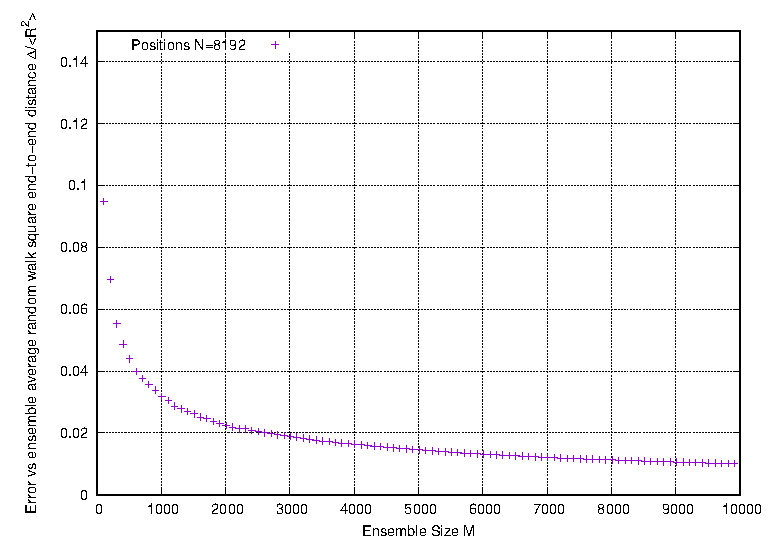
\includegraphics[scale=1.2]{figure1a.eps} 
\end{center}
\caption{Relative error $\Delta / \langle R^2 \rangle$ vs ensemble size $M$ for non-self avoiding 2D continuous random walk.}
\label{fig:1a}
\end{figure}

Also, as figure~\ref{fig:1b} shows, the ensemble average squared end-to-end distance behaves as expected with
$\langle R^2(N) \rangle \propto N$ for $N \rightarrow \infty$.

\begin{figure}[ht]
	\begin{center}
	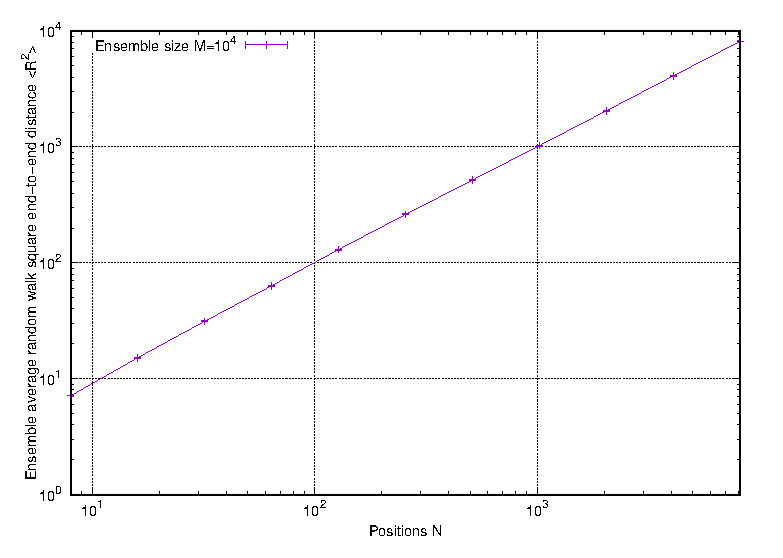
\includegraphics[scale=1.2]{figure1b.eps} 
	\end{center}
	\caption{Ensemble average squared end-to-end distance $\langle R^2(N)\rangle$ vs random walk lenght $N$ for non-self avoiding 2D continuous random walk.}
	\label{fig:1b}
	\end{figure}

\subsection{Task 2}

Now for a self avoiding random walk in three dimensions, the error behaves as in task 1 as $\Delta \propto \frac{\langle R^2 \rangle}{\sqrt{M}}$ for $M \rightarrow \infty$
 as shown in figure~\ref{fig:2a}.

\begin{figure}[ht]
\begin{center}
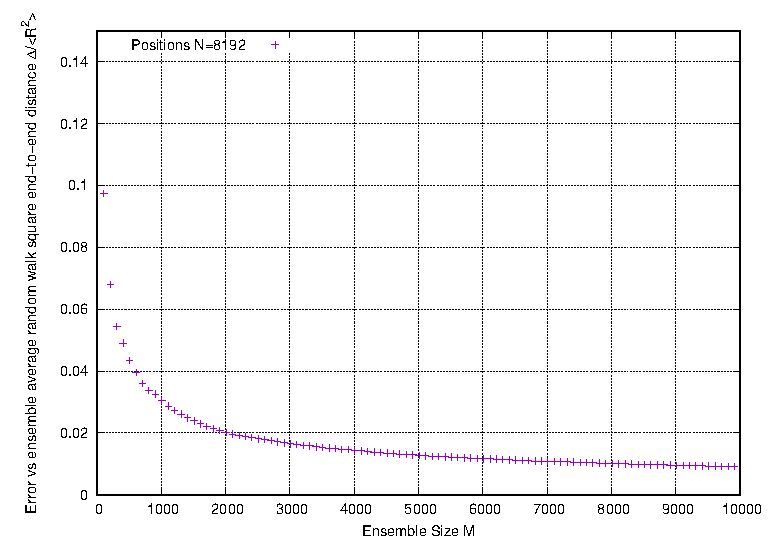
\includegraphics[scale=1.2]{figure2a.eps} 
\end{center}
\caption{Relative error $\Delta / \langle R^2 \rangle$ vs ensemble size $M$ for self avoiding 3D continuous random walk.}
\label{fig:2a}
\end{figure}

blublub

As figure~\ref{fig:2b} shows, the ensemble average squared end-to-end distance no longer behaves as in the non-self avoiding
2D where we had $\langle R^2(N) \rangle \propto N$ for $N \rightarrow \infty$, but seemingly as a power law with an exponent
of slightly above one. This is reflected by the slope of the straight line in figure~\ref{fig:2b}.

\begin{figure}[ht]
	\begin{center}
	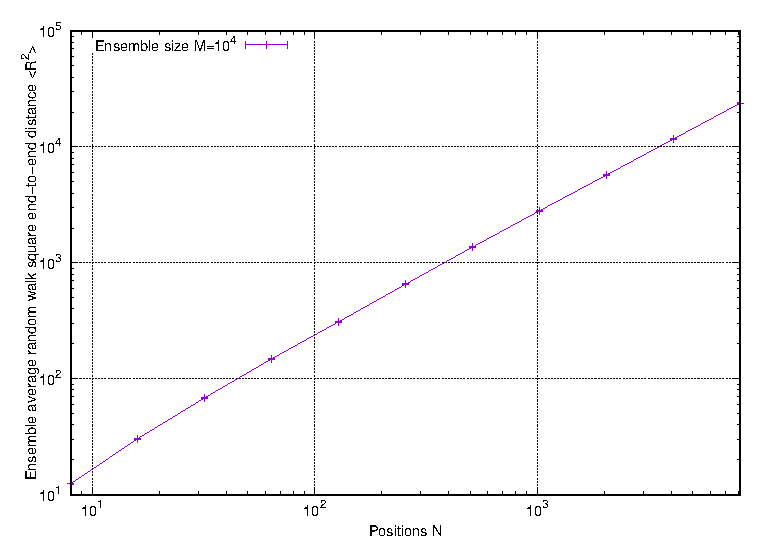
\includegraphics[scale=1.2]{figure2b.eps} 
	\end{center}
	\caption{Ensemble average squared end-to-end distance $\langle R^2(N)\rangle$ vs random walk lenght $N$ for self avoiding 3D continuous random walk.}
	\label{fig:2b}
	\end{figure}



\section{Discussion}
The results were all in line with expectations. To me, the biggest challenge was to write the algorithm such that trapped
walks get thrown away when really stuck but not too early as otherwise the chance to obtain complete walks with larger $N$ 
drops rapidly.

% \begin{thebibliography}{99}


% \bibitem{metropolis}
% Metropolis, N.,
% Rosenbluth, A.W.,
% Rosenbluth, M.N.,
% Teller, A.H.,
% Teller, E.\\
% \emph{Equations of State Calculations by Fast Computing Machines},\\
% Journal of Chemical Physics. 21 (6): 1087,\\
% 1953.


% \bibitem{herrmann}
% 	Herrmann, H. J.,
% 	Singer, H. M.,
% 	Mueller L.,
% 	Buchmann, M.-A.,\\
% 	\emph{Introduction to Computational Physics - Lecture Notes},\\
% 	ETH Zurich,\\
% 	2017.


% \end{thebibliography}

\end{document}